\section{Electronics}
% ============================= Introduction =============================
\subsection{Introduction}
\noindent In the beginning the team was split into three subgroups;

The vision group, two persons working full time on vision. Without vision, no missions above regular movement can be achieved, so getting this system to work was crucial for future development.

The Graphical User Interface (GUI) for mission control, one person working for half the project. This part was made so that a person not knowing much or anything at all about the software inside Naiad should be able to program the missions for the competitions or even real missions in the future.

Naiad main control software, three persons working full time and one person working half time. This group had the responsibility to get Naiad moving correctly, in water and simulations, all nodes on the CAN-bus and that all internal and external communication was working as supposed.

The software system is almost redone from scratch, except some firmware and vision from Vasa and old Naiad. The main reason to redo most of the work was to make the complete system more modular, in the end a node based on Transmission control Protocol (TCP) system which is communicating with JavaScript Object Notation (JSON) \cite{JSON} was built. With this system done, the three subgroups (vision, mission interface and Naiad main control) would make it easier to implement and test their software without having to rebuild the whole system. This also lead to a more agile/scrum like development, due to small nodes which could be done and tested faster, without having to change much or anything at all in the existing system.

On the BeagleBone Black (BBB) \cite{BBB} and CAN-bus all code running is written in Ada, the vision is written in C/C++ and external programs are written in Ada, C\#, Matlab and python. 
For the ease of communicating between the same and different languages, the JSON standard was used over TCP. BBB uses  Universal Asynchronous Receiver/Transmitter (UART) to communicating to a CAN-node connected to the CAN-bus that joins everything to one system.

Robustness and reliability are key components in a robot, so most code in Ada has been written taking Ravenscar \cite{Ravenscar} in consideration. Some fail detection is also implemented in the CAN-bus to be able to restart the system if needed. The BBB main routing node can also check what other nodes is connected.

To achieve an greater form of modularity, space plug and play avionics\cite{spnp} have been started to be implemented, as for now when a new CAN-node connects, it will send its name to the power supply unit(PSU) CAN-card, this information will then be passed on to the BBB, this can also be done on request, so that the PSU CAN-card asks the system what cards is still connected, gather the information and send it to the BBB.


\begin{figure}[!ht]
	\begin{center}
		\includegraphics[width=80mm]{./Images/Software/flowchart.png}
		\caption{Complete flowchart of software}
		\label{YourLabel}
	\end{center}
\end{figure}
 %Written by Anette
	
% ============================= Background =============================
\subsection{Background} 
  When the project started this year a lot of the fundamental electronics had already been created. This meant that the overall electronic design was decided as well as thrusters and motor-drivers. The power supply was complete as well as the base of the Controller Area Network (CAN) bus. The Microcontroller unit (MCU) AT90CAN128 was decided as a CAN-bus control unit and stacks to mount and connect the cards was complete. There are a lot of redundancy in the system, for example, each CAN-card transforms from 24 to 5V. An explanation for this from the previous team was to increase robustness in the system. If a leakage occurs and the 5V on the power board and 24V is shortened the CAN-card will not burn. Each CAN-card can handle 12.6-48V making them less sensitive to spikes in the system than if one 5V source would go straight in to all of the MCUs.
  
  	\subsubsection{Generic CAN} %Anette
From the previous team, a generic CAN-card was created that has the version number 4.4. This card has nine analogue and eight digital IO-channels. As well as SPI, two UART channels and CAN-bus interface. The card is equipped with a AT90CAN128 MCU giving each card its own computing power. This makes it possible for the card to interpreted CAN-messages, make computation and give out an response. There was a requirement from last year that all of the sensors were to have its own computing power. This requirement was removed during this project. For the most part the card is fully functional. There are some bugs still though. For example the footprint for the 100nF electrolyte capacitor to the left of the switched DC-DC converter is backwards. This can be seen in fig. \ref{Capacitor}

\begin{figure}[!ht]
	\begin{center}
		\includegraphics[width=90mm]{./images/Electronics/Capasitor.jpg}
		\caption{The capacitor marked C12 have an incorrect footprint, the footprint is backwards compared to the shoe on the capacitor.}
		\label{Capacitor}
	\end{center}
\end{figure}
   
	\subsubsection{Thrusters} %Patrik
\noindent
The previous team had decided to use the Crustcrawler 400HFS thrusters\cite{thrusters}. They are specially designed for AUV and ROV applications, and are, compared to their size, quite powerful. We had no reason to question this decision since they were already mounted and running. The motors were controlled by the Phoenix Ice2 HV 60 motor controller from Castle Creations \cite{motor_drivers}. The drivers, originally designed for RC air crafts, were bought with custom built firmware, designed to be able to instantly switch rotational direction. The previous team had not been able to get the special firmware settings to work.
 
		\subsubsection{Stack}
	To connect and support the CAN-cards a board that makes it possible to stack these on top of each other was created last year. These holders could hold three cards and the cards was soldered to the stacks. This created some problems with fitting add-on cards. Also if a card would break it was difficult to replace unless all three cards was replaced. 
	
	\subsubsection{Power supply unit} %Anette
A power supply unit (PSU) existed, which was created to supply the different parts of the system from a single source. This card have not been changed during this project. A CAN-card on the PSU can control the supply to different parts of the system. The only thing that can not be control entirely by the software on the CAN card is the supply to the motors. For the thrusters to be supplied the they need to be enabled by the card but the kill-switch also need to activated. The kill switch consists of two physical pins than need to be connected in order to supply the motors. This switch can not be overwritten or controlled in software but are built in to the board. The kill switch controls the power to the thrusters as well as the 12V output but \emph{not} the rest of the system. The CAN-bus and 5V output can be started even if these pins are not connected. There are a few patches on the card printed from Würth electronics. These patches has been added to the schematics but no board design has been made. The schematics is backward constructed from the physical card since proper documentation was absent from the previous group. Even though it has been proofed several times there might still be errors it it. To read more on how the card works see appendix \ref{A_powerboard}. The schematics can be found in appendix \ref{Schematics_Power}.

	\subsubsection{Inertial Navigation System board} %Lennie
When the previous group was working on Naiad the design of the Inertial Navigation System (INS) board was started. A design was proposed for the Fiber Optical Gyroscope (FOG) and was built but not tested. During the summer there was another electronics project where one person had as a mission to test the INS board and discovered that it did not work. The design was not working properly, since the circuit was not complete. Instead it worked as an current generator. A new design was proposed during the summer project and a lot of tips for improving the card was proposed. The proposed board was not built so the design ideas could not be tested. During this years project the ideas was taken into account. Improvements was then made and a new card was built and have been undergoing testing.
	 %Written by different people

% ============================= Gen CAN =============================
\subsection{Generic CAN} %Anette
The generic CAN-cards from the previous group can handle several kinds of signals. This is a good base but to effectively use the cards features additional peripheral electronics are required. Therefore shields or add-on cards for these CAN-cards to add functionality to them has been created.  These add-on cards are discussed in more detail in their separate sections. 
In the beginning it was sufficient to only do these add-on cards to the old CAN cards. When it was decided to save space by controlling several motor controllers on one card, it was discovered that the PWM signals on the old card was insufficient both in number and in resolution. It was therefore decided to make a new generation of the card. This time with six high quality PWM signals since the MCU could provide this but at the moment these outputs were not connected. 

To speed up the process of creating this card, as much as possible was kept from version 4.4. At the time the card was redone, no schematics of the card was available but the board-design file was accessible. The required traces were simply re-drawn and the rest left as is. The user-LED, a LED that can be controlled in software, was occupying one of the high quality PWM signals from the MCU. It was therefore moved from MCU pin 6 to pin 14. After miscommunication in the group it was believed that the SPI interface were not used and was therefore removed in version 5.0. 

It is believed that it is possible to keep the SPI in future generations. By moving the two PWM signals that are currently located where the SPI used to be in 4.4 to the other side of the 5V (where the M\_PWM are located on version 4.4). This would require the motor extension board and the LED-control board to be modified as well. If this was done the same card should be able to be used on all locations of the system adding to the robustness of the system and require less spare parts to be brought to San Diego. At the moment both version 4.4 and version 5.0 are in the system.
%referea till scematics 
%The 4.4 version as an error in the silk screen of the electrolyte condensator 
%NEW STACKS FOR THE CARDS
	
	
% The incorrect footprint of electrolyte capacitors
% 5.0 has been "printed" without silc screen %Written by Anette

% ============================= Gen CAN =============================
\subsection{Stacks} %Anette
The stacks from the previous group were replaced with stacks that had connectors on them to increase flexibility. The connector used is a four pin bottom entry socket header from Würth electronics. The headers are placed on the back of the stack and the CAN-cards need to be inserted \emph{through} the card and the header. Otherwise the connections will not line up properly. The break away headers on the CAN-card need to be angled and longer than standard. The pins need to go through both card and connector and show on the back on order to make a secure fit. These stacks have 4 levels. Not all are intended to be used at the same time. This is due to size and space. There is nothing in the electronics that limits that all connections are used at once. The levels are there as redundancy as well as making it more versatile. If extra stability is decried the two pins to next to the power supply are not connected on any level and can be used as extra support.
	%Make new healder not in background  %Written by Anette

% ============================= INS-board =============================
\subsection{INS board}
The INS board is powered and delivers navigational data to a CAN-card. It delivers the data that the Inertial Measuring Unit(IMU) measures through a USART interface to the CAN card. It also measure values from the Fiber Optical Gyroscope(FOG) and sends it from the INS board to the CAN-card through a SPI interface. The INS board also offer the FOG the safe and stable power levels it requires. The FOG is very sensitive to voltage levels, especially when it comes to the 5V, 12V \& -12V lines, there are safety solutions implemented. As an example, to start the 5V three requirements needs to be fulfilled. A digital pin needs to be set high through software and the 12V \& -12V lines need to be active. This is because the FOG might break if the 5V power is on without $\pm$12V being active. When these requirements are fulfilled the FOG is active and the INS board can start supplying data to the CAN-card.
	
 %Written by Lennie
	
% ============================= LED-control board =============================
\subsection{LED controller}
The LED controller board is made to control all the lights. Naiad will have two sets of light containing two regular and one ir-headlight. One pointing forward and one downward. It will also have two RGB LEDs on each wing to make it easier to understand decisions made by Naiad. The LED card has two power supplies. One from the PSU powering the LEDs and one from the CAN-card powering the logical circuit. The RGB LEDs on the wings is controlled by a CAN-card through a SPI interface. To activate an LED 16 bits needs to be sent. The headlights is controlled by a PWM signal. One PWM signal for the headlights facing forward and one for the headlights facing downwards. The duty cycle of the PWM signal determines the brightness of the headlights. The experimental LED-controller board can be seen in fig. \ref{LedImgText}.

\begin{figure}[!ht]
	\begin{center}
		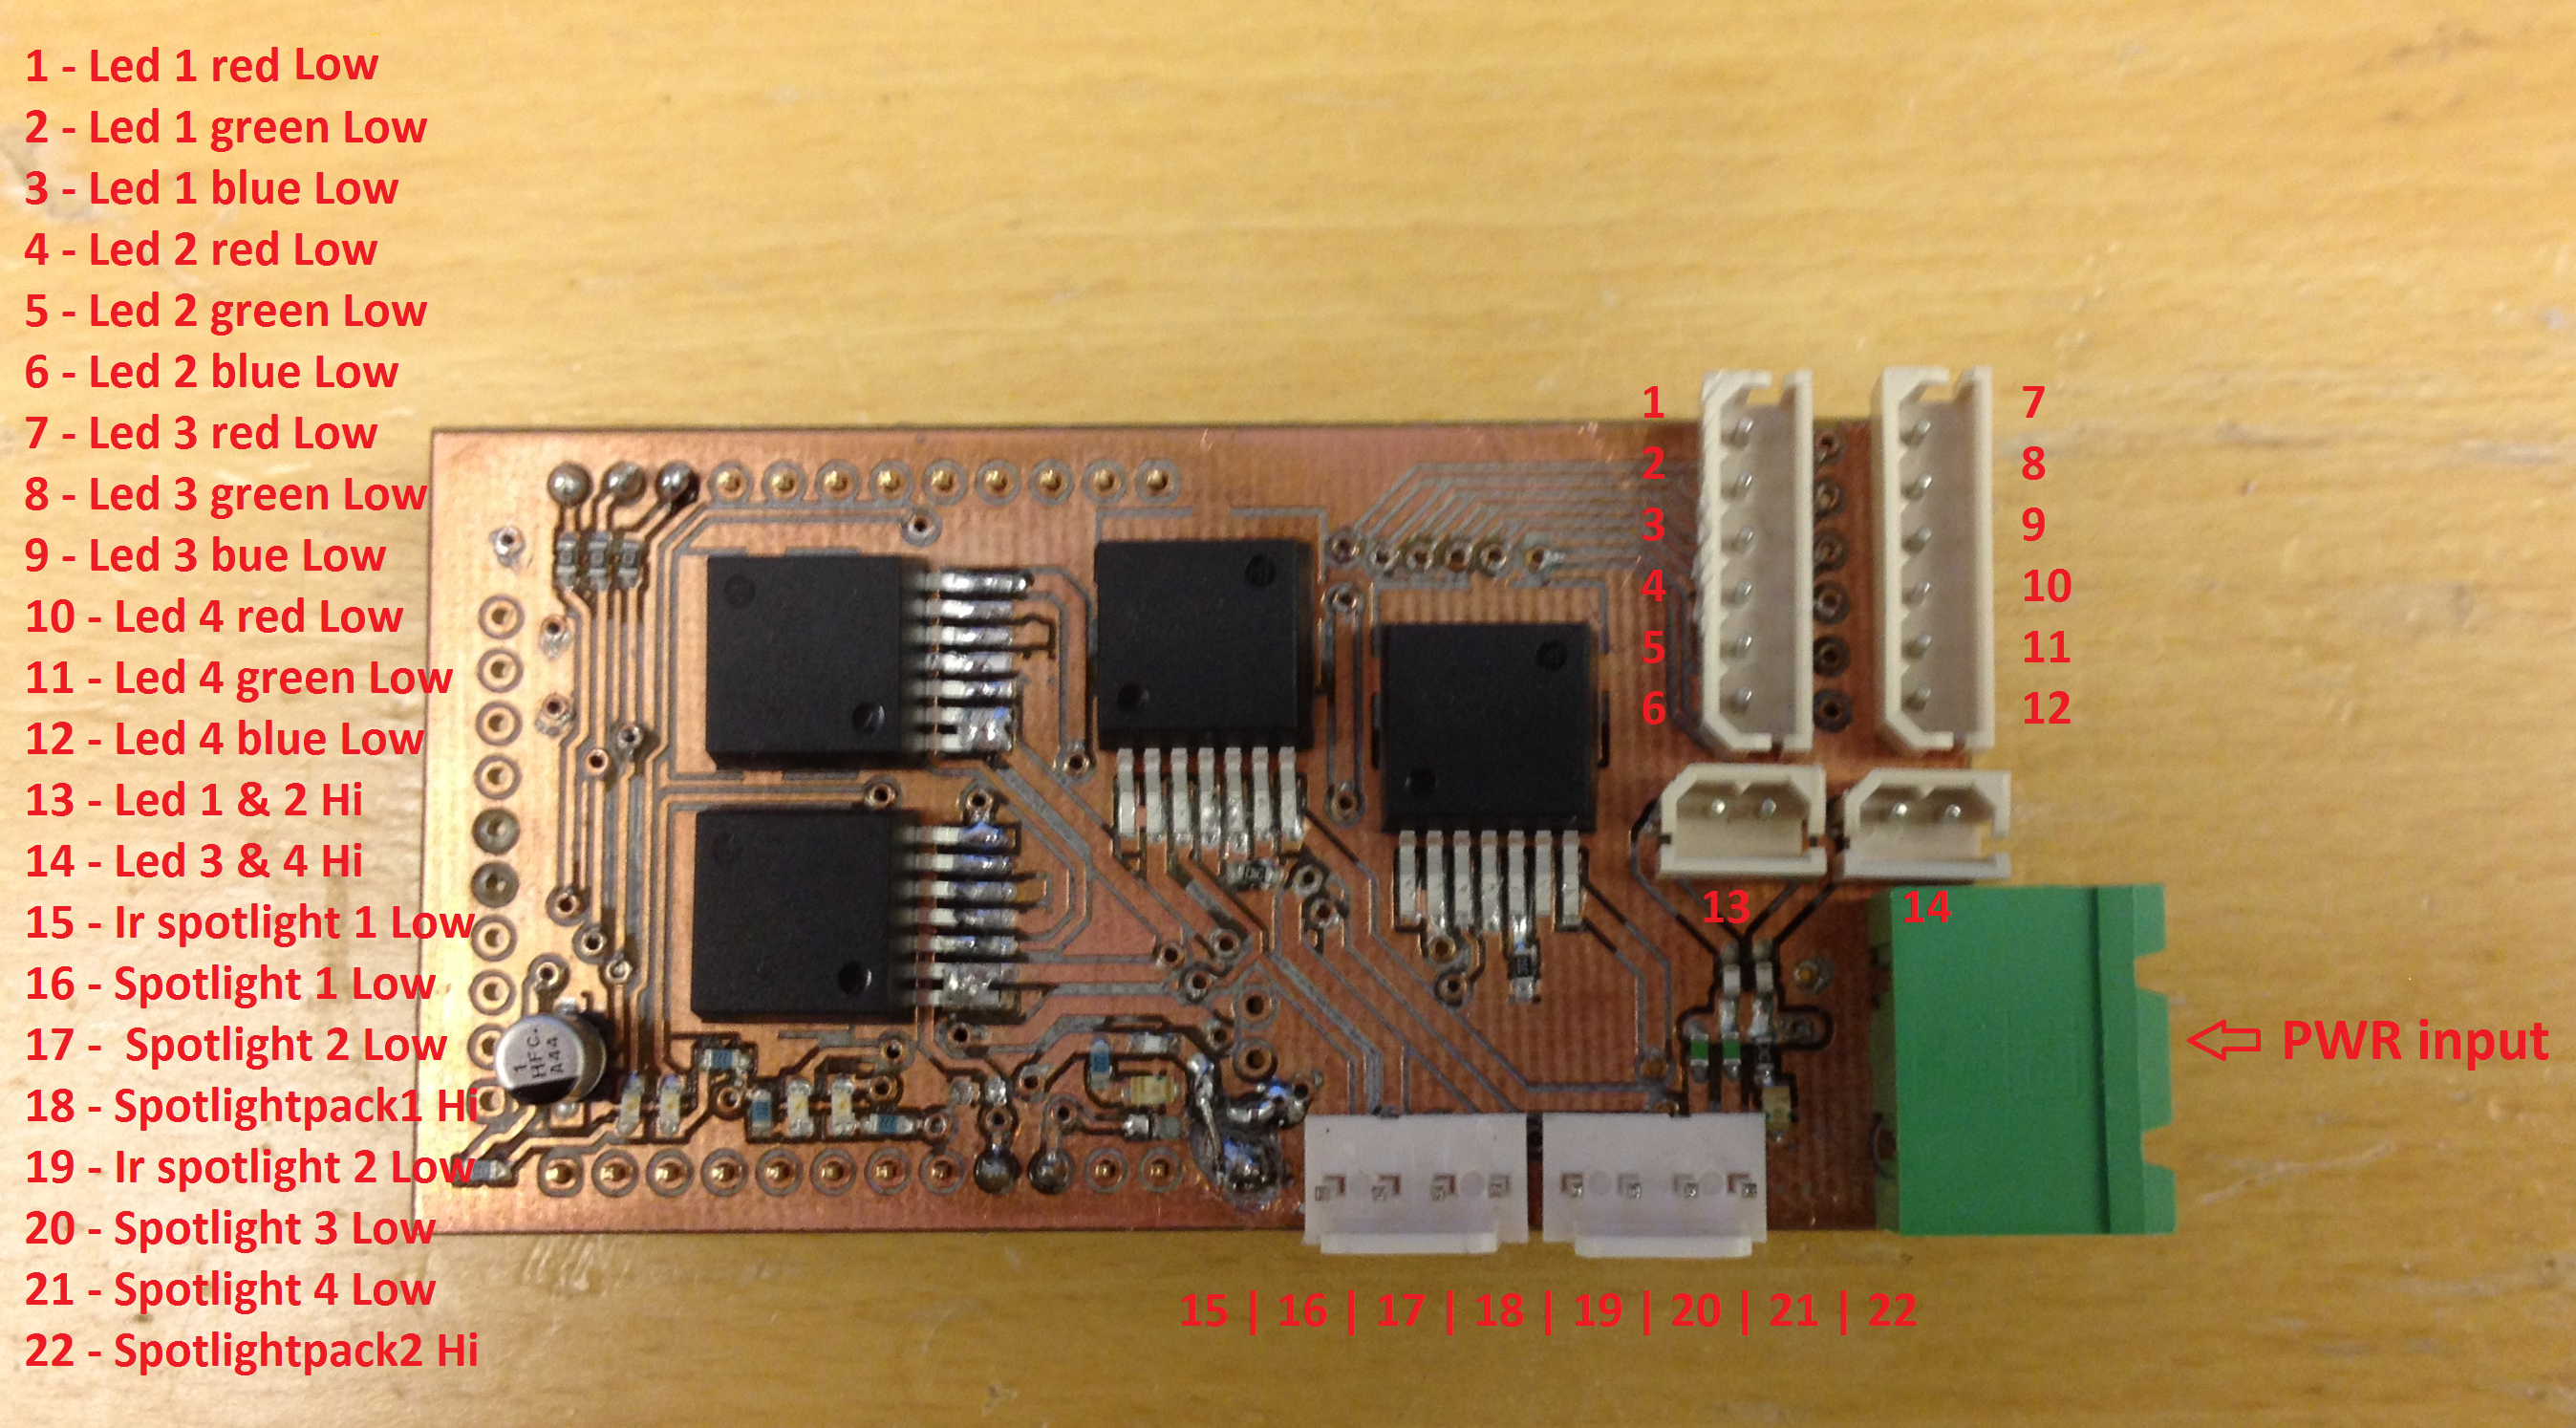
\includegraphics[width=80mm]{./Images/Electronics/LedImgtext.png}
		\caption{Picture of the experimental LED controller board}
		\label{LedImgText}
	\end{center}
\end{figure}

	
 %Written by Lennie

% ============================= Hydrophone =============================
\subsection{Hydrophone} %Patrik
\noindent
One of the missions in the RoboSub competition is to locate the resurfacing point. This location is marked with an acoustic pinger, located at the bottom of the pool underneath the exit site. The pinger sends out a 4 millisecond ultrasonic beep every 2 seconds \cite{robosubrules}. To determine the location of the pinger, four hydrophones are used to determine the direction the sound is coming from. By comparing the differences in time when the hydrophones hears the ping, a direction towards the source can be calculated. The reason for four hydrophones is that, to be able to locate a source in the 3 dimensions, observation of the signal will also be needed in 3 dimensions. With three hydrophones you would be able to get the the angle to the object in the plane, but not know how far off the plane the source is. This setup might have worked in the competition, with the pinger located on the bottom. Since the Naiad is built for a more general purpose, an exact direction in three dimensions is more usable in future applications.

The sound from the pinger needs to be drastically amplified in order for the MCU to handle the signal.The water is not a silent place, so the signal has to be filtered in order to pick up the desired frequency. This is done by the hydrophone shield card, which picks up the signals from the four hydrophones. The card has three main tasks:
\begin{itemize}
\item{Phantom power}
\\The hydrophones gives a much more desirable signal if they are supplied with a constant voltage. This is a done by a voltage division and a big capacitor for stabilization. This power supply can be used for all four hydrophones.
\item{Filter and amplification}
\\The signal runs through a passive high pass filter with a tunable cut off frequency. It is able to filter out frequencies below 10-50 kHz. After the filtering the signal is amplified in two stages. After an  initial amplification the signal is split. One unaltered signal is buffered. Another signal is used as reference voltage for the last amplification stage. These signals are fed as input to the last amplification, where the difference between these two signals are amplified almost 200 000 times to get a clear input to the mcu .
\item{Digitalization and voltage restriction} \\
After the final amplification, the signal is smoothend to a digital high by a capacitor and picked up by one of the interrupt pins on the CAN-card.

\end{itemize}

No equipment for testing the circuit properly has been available. The pinger in the lab is limited to 20kHz and the circuit has worked at close range. No open water test has been conducted. The motors rattle and make a lot of loud noises. Since these sounds origins from a source very close to the hydrophones and the sounds are built from a wide range of frequencies, the sound is almost impossible to filter away, at least with the analog filter approach. Therefor, the only way to pick up the sound from the pinger is to turn the thrusters off and listen, whilst dead in the water.

A digital filter was ruled out due to lack of funds, time and hardware with high enough sampling frequency. The digital filter, with way sharper edges, may have been able to listen for the pings and completely remove any noise from the motors.  	
 %Written by Patrik

% ============================= Speed logger =============================
\subsection{Speed-logger} %Patrik
\noindent
The purpose and mechanical design of the speed logger can be found in section \ref{SL_mec}. The electronics parts of it is divided to an outer sensor and an inner analysing circuit.

\subsubsection{Sensor}
\noindent
The sensor is based on two Allegro A1301 hall sensors. They translates differences in the magnetic field to analogue voltages. These are placed side by side with 5 mm spacing on a small PCB near the rotating turbine. 
The propeller has magnets mounted on its blades, and by reading the timing differences between the sensors, rotational direction and speed can be determined.

\subsubsection{Circuit}
\noindent
The signal from from the sensors needs to be altered in order to work as an interrupt edge for the responsible CAN-card.
The IC circuits on the sensor has a default voltage of half of the supply voltage.
To get an accurate reference voltage, a third A1301 sensor is used inside the hull as a reference voltage.
The difference between the inside and outside sensors is amplified in order to trigger the interrupt on the MCU. 

	
	
 %Written by Patrik

% ============================= Motor extension board =============================
\subsection{Motor configurations}
\subsubsection{Motor extension board} %Anette
The motor extensions board is, in it essence, an adapter. It provides the motor controller with 5V and GND from the CAN card as well as a PWM signal in a suitable connector. It has six three pin WR-WTB connectors from Würth electronics, one for each motor controller. These were chosen since they prevent the user from connecting the cable upside down and is also has a locking mechanism. The current version of the board is made to be used with the 5.0 CAN-card.

\subsubsection{Motor controllers} %Patrik
The controllers was configured with the Castle Link V3.52.10 software. The reason the previous team had trouble with it was that since the firmware was altered from the supplier, some of the files for the setup program had to be replaced. The software is able to configure a number of thruster settings, one of which is the reverse type. The "crawler reverse" setting enables the motors to rapidly change rotational direction in order to make the AUV more agile. %Written by Anette

% ============================= Remote controller =============================
\subsection{Remote control}
When the lid is closed and the Ethernet cable is not plugged in to Naiad there is no easy way to change settings. The remote controller is made to work on land. With the remote control one can navigate and change settings presented on the LCD display. The remote has 4 buttons and one slide switch. The four buttons is for navigating through the menu and the switch is for turning the remote on or off. Since there are no power saving function built in, the batteries in the remote controller will only last for 24 hours unless the switch is turned off after use. The remote uses a commercially bought transmitter and receiver circuit for sending data on the 433MHz FM band. %Written by Lennie

% ============================= Sensor board =============================
\subsection{Actuator board} %Lennie
The actuator board is a board made to control the solenoids for the markers and the torpedoes. The board can have one or two inputs and four outputs. One input can power either two or four actuators depending if the two pins located below the fuses named pwr\_bridge is bridged. The power inputs can be at any level between 0V to 24V. The actuator board does not have any current regulators for the outputs, this is because each output will only be activated for a short time, when the markers get dropped or torpedoes shot. The solenoids that the outputs will power will also be submerged in water, so the heat will not be a problem. Each solenoids is controlled by a digital high/low signal that is sent from a CAN-card. The experimenal actuator board can be seen in fig. \ref{ActuatorImgText}.

\begin{figure}[!ht]
	\begin{center}
		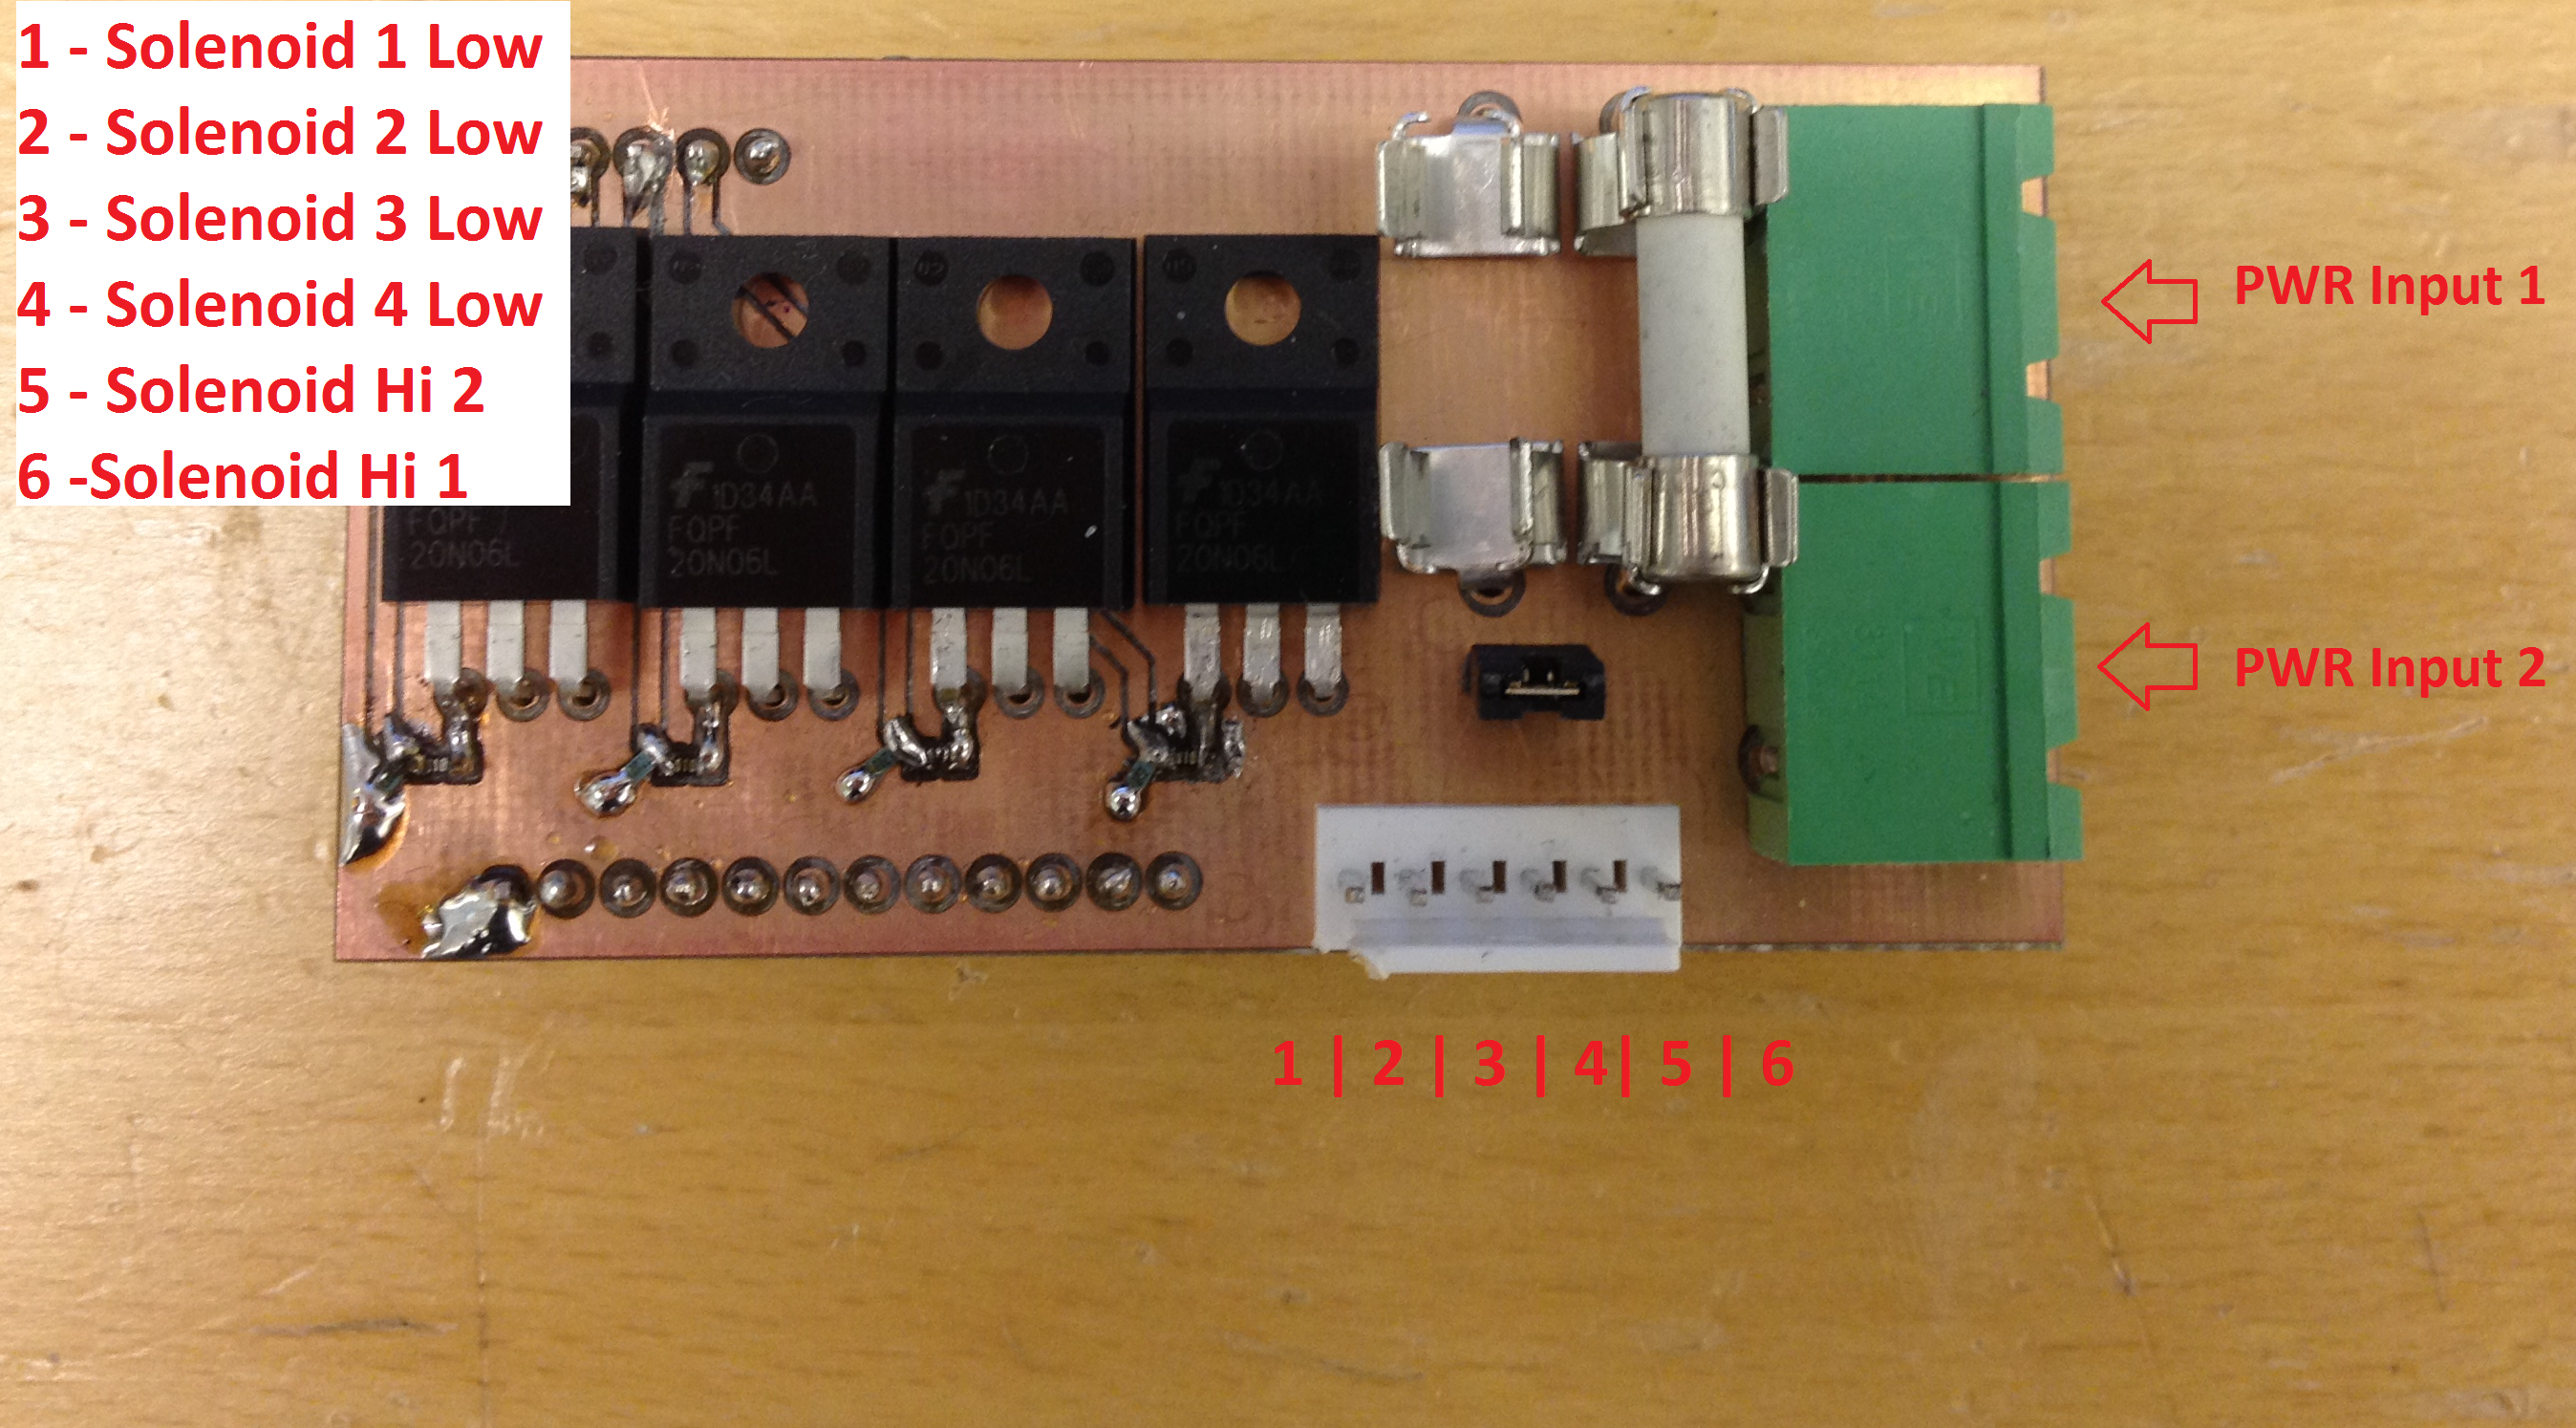
\includegraphics[width=80mm]{./Images/Electronics/ActuatorImgText.png}
		\caption{Picture of the experimental actuator board}
		\label{ActuatorImgText}
	\end{center}
\end{figure}


	
 %Written by Patrik

	
	
